\subsection{Regression}

\begin{definition} \hlt{Linear Regression Assumptions}
\begin{enumerate}[label=\roman*.]
\setlength{\itemsep}{0pt}
\item Linearity: $Y \sim a_i X_i$, where $a_i$ is a constant, $Y$ is dependent variable, $X_i$ is independent variable.
\item Homoscedasticity: Variance of residual $Var(Y - \hat{Y})$ is constant $\forall$ observations ($Y$ is actual, $\hat{Y}$ is predicted).
\item Independence: Residuals are uncorrelated across observations, $E[\epsilon_i \epsilon_j] = 0 \ \forall i \neq j$.
\item Normality: Residual term is normally distributed. 
\item Expected value of residual term is zero, $E[\epsilon] = 0$.
\item Independent variable is uncorrelated with the residuals.
\end{enumerate}
\end{definition}

\begin{definition} \hlt{Regression Performance Plots}:
\begin{enumerate}[label=\roman*.]
\setlength{\itemsep}{0pt}
\item Scatterplot (variable vs variable): for possible correlation between independent variables, identify outliers.
\item Scatterplot (residual vs predicted): for possible correlation between residual and predict value.
\item Normal Q-Q plot (theory vs empirical distribution): residual vs normal distribution. If residuals are along the diagonal, then it is good.
\end{enumerate}
\end{definition}

\begin{definition} The estimated \hlt{slope coefficient} $\hat{b}_1$ is computed as $\hat{b}_1 = \frac{Cov(X,Y)}{\sigma_X^2}$.
\end{definition}

\begin{definition}The \hlt{standard error (SE)} is defined as $SE = \frac{\sigma}{\sqrt{n}}$.
\end{definition}

\begin{definition} The \hlt{regression coefficient confidence interval} is defined as $\hat{b}_1 \pm (t_{\alpha} + SE_{\hat{b}_1})$, where $t_{\alpha}$ is the critical two-tailed t-value for the confidence level $\alpha$, with degrees of freedom $df = n-2$.
\end{definition}

\begin{definition} \hlt{Test of Slope Coefficient Significance}\\
Two-tailed test $H_0: b_1 = 0$ against $H_{\alpha} : b_1 \neq 0$.\\
Test statistic is $t = \frac{\hat{b}_1 - b_1}{SE_{\hat{b}_1}}$, with degrees of freedom $df = n-2$.\\
Reject $H_0$ if $t > t_{\alpha/2}$ or $t < - t_{\alpha/2}$.
\end{definition}

\begin{figure}[H]
\centering
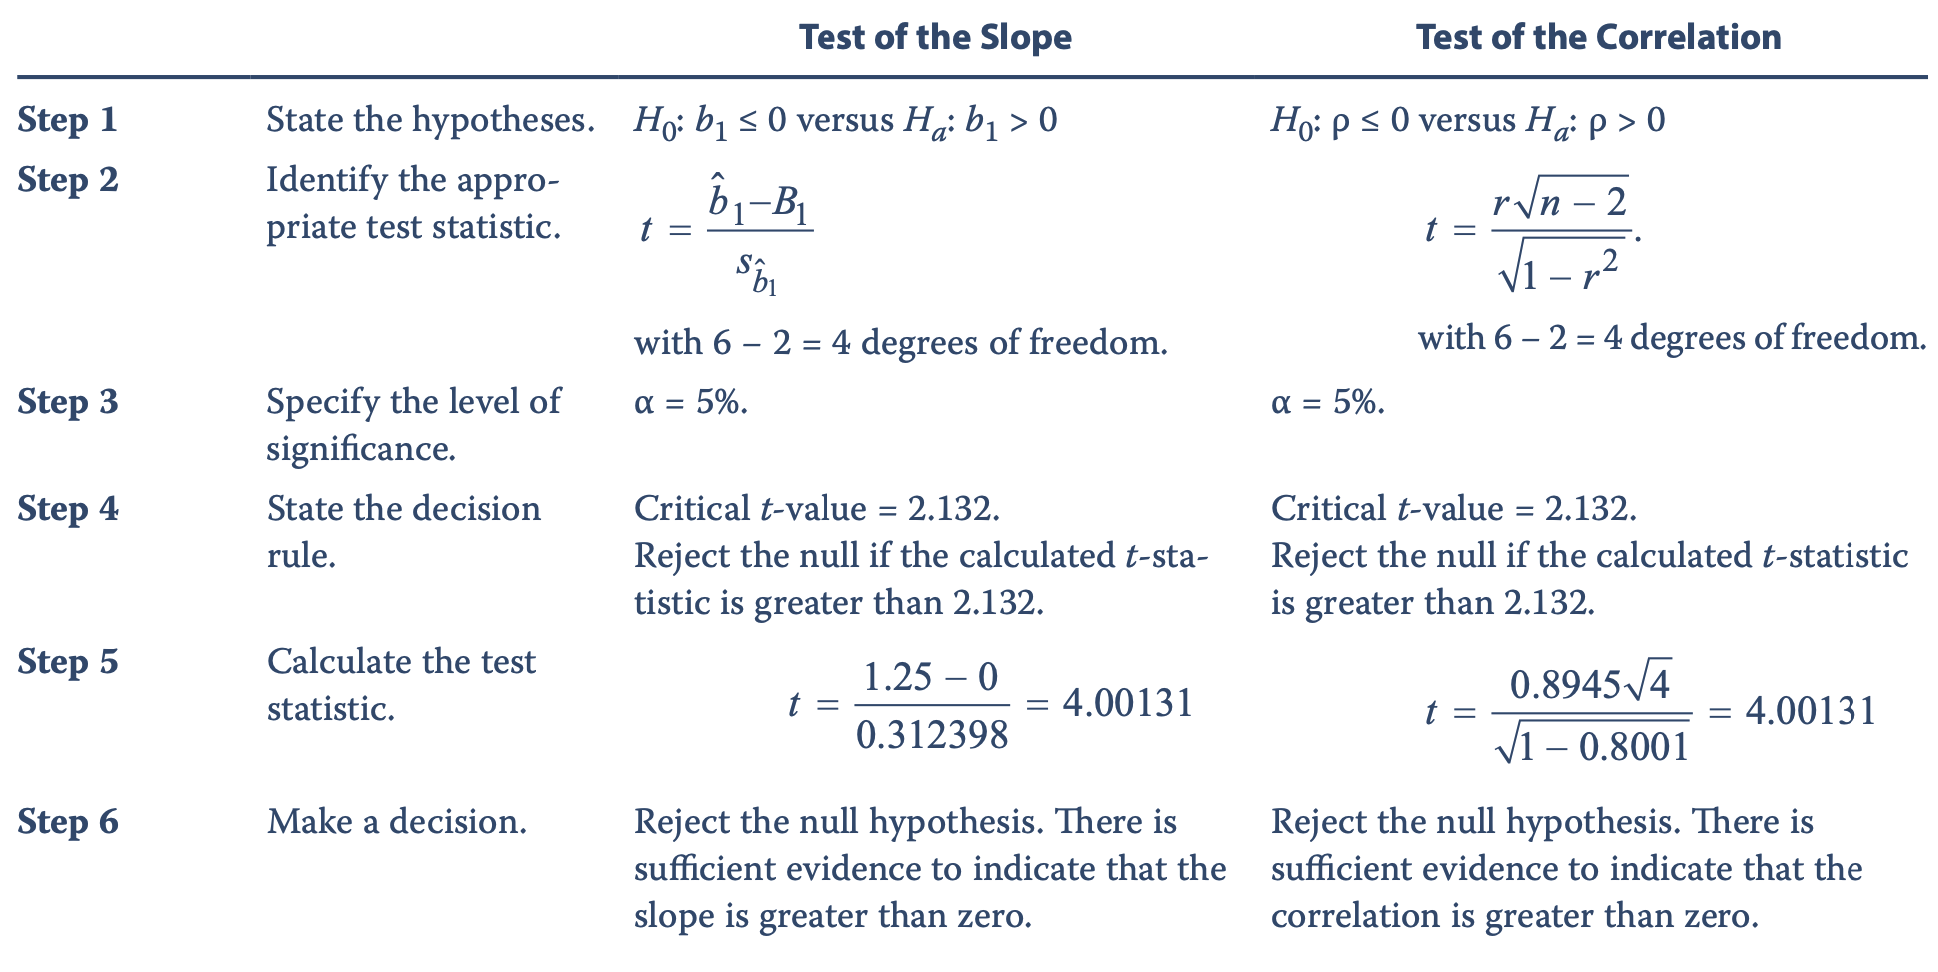
\includegraphics[scale=0.5]{quant/onesidetest}
\caption{One-sided tests for slop and correlation, single regression}
\end{figure}

\begin{definition} The \hlt{predicted values confidence interval} is defined as $\hat{Y} \pm (t_{\alpha/2} \times SE_{f})$, where $t_{\alpha/2}$ is the critical two-tailed t-value for the confidence level $\alpha$, with degrees of freedom $df = n-2$, and $SE_f$ is the standard error of the forecast. 
 Note that $SE_f^2 = SEE^2 \left[1 + \frac{1}{n} + \frac{(X - \overline{X})^2}{(n-1)\sigma^2_X} \right]$, where $\sigma^2_X$ is the variance of the independent variable, $X$ is the value of the independent variable for which the forecast was made.
\end{definition}

\begin{figure}[H]
\centering
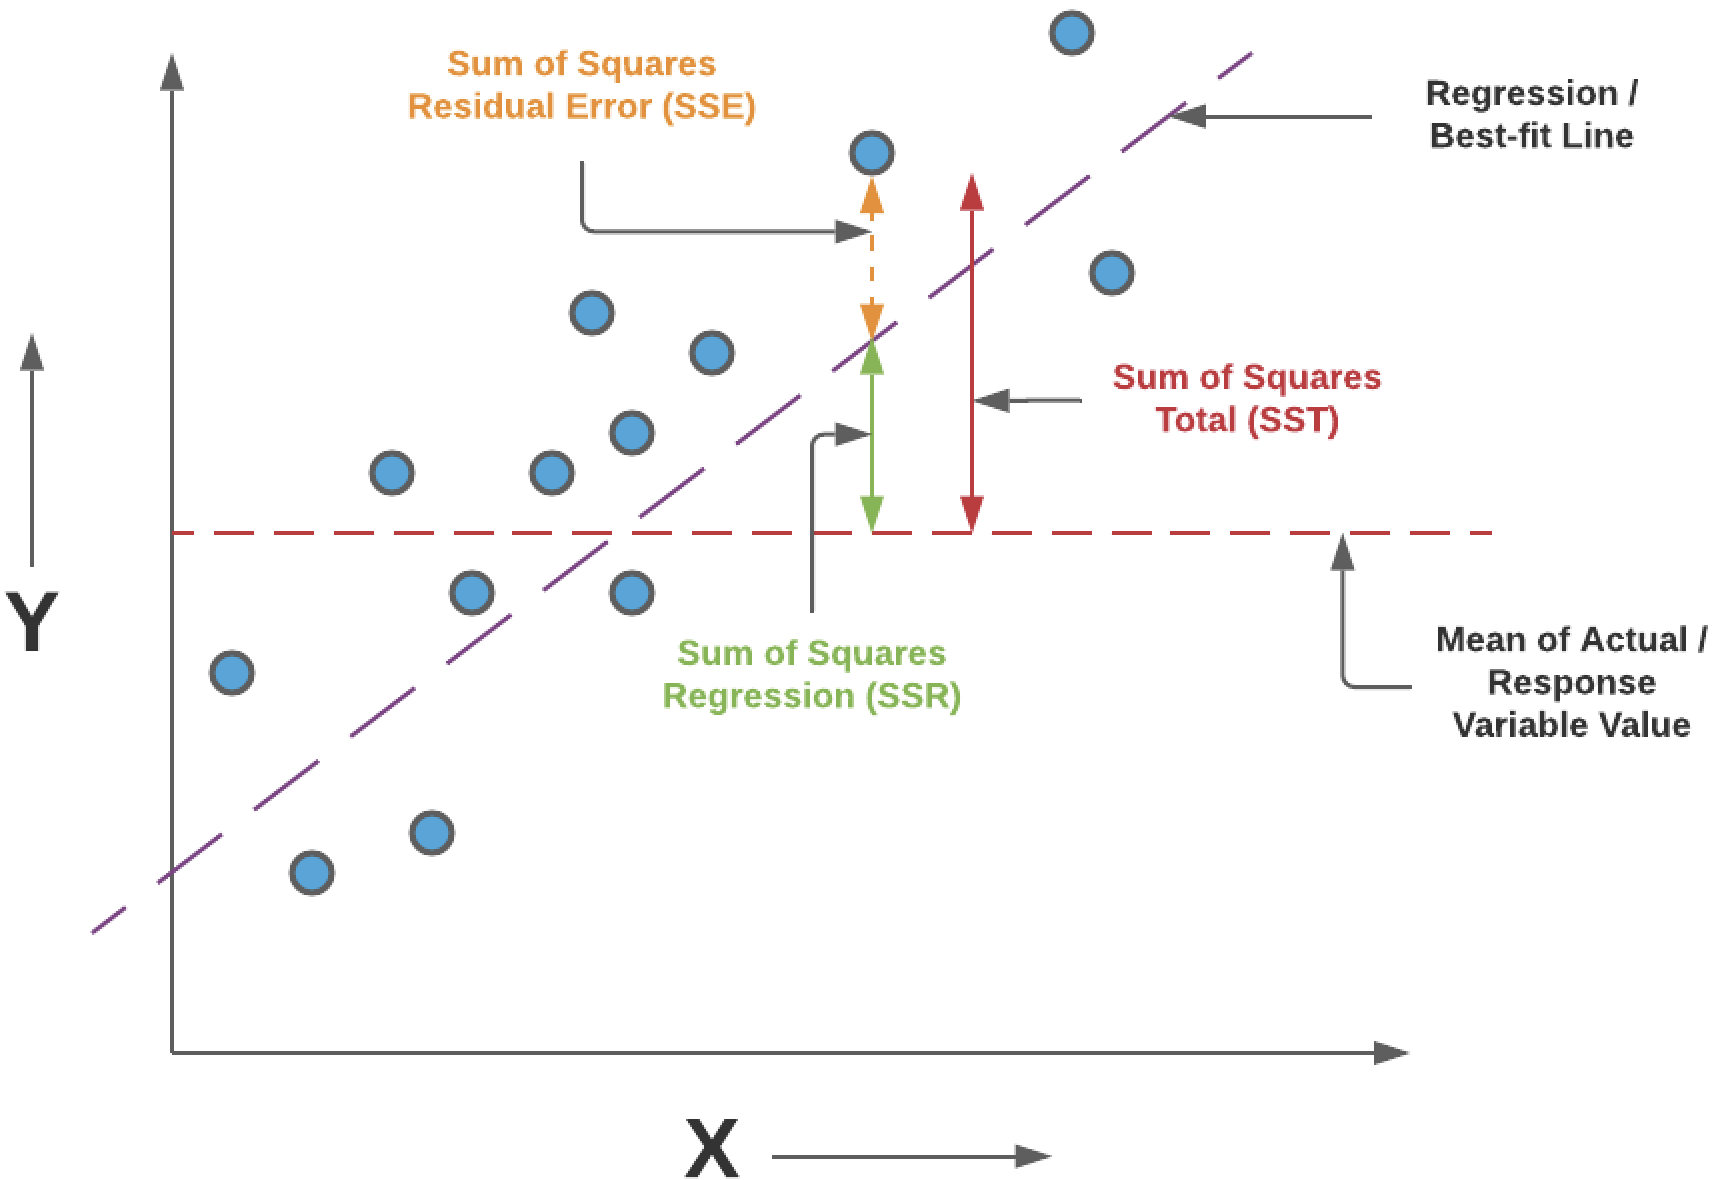
\includegraphics[scale=0.25]{quant/ssr}
\caption{Regression Error Terms}
\end{figure}
 
\begin{definition} \hlt{Analysis of Variance (ANOVA)} analyses the total variability of the dependent variable:
\begin{enumerate}[label=\roman*.]
\setlength{\itemsep}{0pt}
\item Sum of total squares (SST): measures total variation in dependent variable. Sum of squared differences between actual and mean value, $SST = \sum\limits_{i=1}^n (Y_i - \overline{Y})^2$.
\item Sum of squares regression (SSR): measures variation in dependent variable as explained by independent variable. Sum of square distances between predicted and mean value, $SSR = \sum\limits_{i=1}^n (\hat{Y}_i - \overline{Y})^2$.
\item Sum of squares residual error (SSE): measures unexplained variation in dependent variable. Sum of squared vertical distance between actual and predicted values. $SSE = \sum\limits_{i=1}^n (Y_i - \hat{Y})^2$.
\item Mean squares regression (MSR): $MSR = \frac{SSR}{k}$, where $k$ is number of independent variables.
\item Mean squares error (MSE): $MSE = \frac{SSE}{n-k-1}$, where $k$ is number of independent variables.
\item Standard error of estimate (SEE): $SEE = \sqrt{\frac{\sum\limits_{i=1}^n (Y_i - \hat{Y})}{n-2}} = \sqrt{MSE}$.
\item Standard error of intercept: $SE_{\hat{b}_0} = \sqrt{\frac{1}{n} + \frac{\overline{X}^2}{\sum\limits_{i=1}^n(X_i - \overline{X})^2}}$
\end{enumerate}
\end{definition}

\begin{definition} \hlt{Test of Slope Intercept Significance}\\
Two-tailed test $H_0: b_0 \leq B_0$ against $H_{\alpha} : b_0 > B_0$.\\
Test statistic is $t = \frac{\hat{b}_0 - B_0}{SE_{\hat{b}_0}}$, with degrees of freedom $df = n-2$.\\
Reject $H_0$ if $t > t_{\alpha}$.
\end{definition}

\begin{figure}[H]
\centering
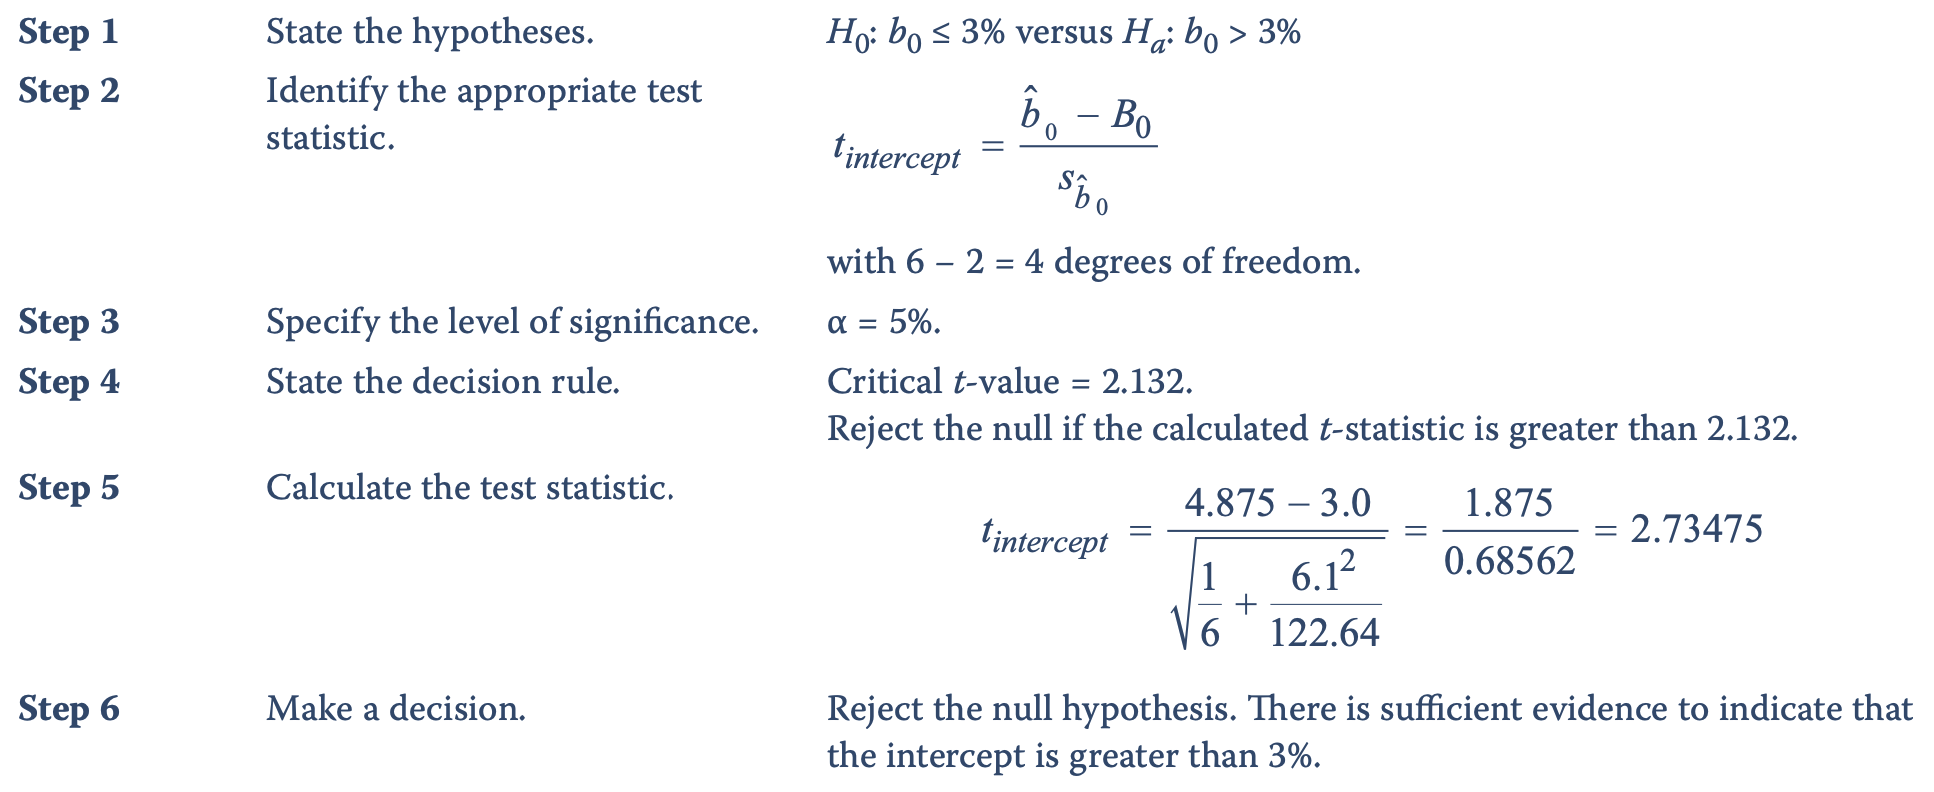
\includegraphics[scale=0.5]{quant/slopeintercept}
\caption{Slope intercept test of regression}
\end{figure}

\begin{definition} \hlt{Coefficient of determination, $R^2$}, measure goodness of fit of regression to data.
\begin{equation}
R^2 = \frac{SST - SSE}{SST} = \frac{SSR}{SST} \nonumber
\end{equation}
\end{definition}

Note that $R^2$ do not allow us to know if coefficients are statistically significant. There is no info on bias in estimated coefficients and predicted values. There is no info if model fit is good as well.

\begin{definition} \hlt{Adjusted $R^2$}, adjusts for degrees of freedom.
\begin{equation}
\overline{R}^2 = 1 - \left[\left(\frac{n-1}{n-k-1} (1-R^2) \right) \right] \nonumber
\end{equation}
where $k$ is number of independent variables.
\end{definition}

If we are adding new independent variable to the regression, if the coefficient t-statistics $> \abs{1.0}$, then $\overline{R}^2$ will increase. If coefficient t-statistics $< \abs{1.0}$, then $\overline{R}^2$ will decrease.

\begin{definition} \hlt{Information Criterions}
\begin{enumerate}[label=\roman*.]
\setlength{\itemsep}{0pt}
\item \hlt{Akaike Information Criterion (AIC)}: evaluate model parsimony. Lower AIC means better fitting.
\begin{equation}
AIC = n \ln(\frac{SSE}{n}) + 2(k+1) \nonumber
\end{equation}
where $n$ is the sample size, k is number of independent variables.
\item \hlt{Bayesian Information Criterion (BIC)}: gives greater penalty than AIC if model has more parameters. Lower BIC means better fitting.
\begin{equation}
BIC = n \ln(\frac{SSE}{n}) + \ln(n)(k+1) \nonumber
\end{equation}
\end{enumerate}
\end{definition}

AIC is preferred if model is used for prediction. BIC is preferred if best goodness of fit is desired.
